%%-----------Chapters start-------------------------------------
%%-----------Chapter 1------------------------------------------
% \documentclass[../UNBThesis2.tex]{subfiles}
\setlength{\parindent}{2em}
% \begin{document}
\chapter{Introduction}
%\setcounter{secnumdepth}{3} \pagenumbering{arabic}
%\setcounter{page}{1} \pagestyle{myheadings}
%\markboth{}{}\markright{} \rhead{\thepage} \setcounter{page}{1}
%\pagestyle{myheadings} \pagenumbering{arabic} \rhead{\thepage}
%\setcounter{page}{1}

%%%%%%%%%%%%%%%%%%%%%%%%%%%%%%%%%%%%%%%%
% Good summary for the introduction
%Data stream affinity propagation algorithm has been chosen for indoor localization data in this research work. For this algorithm, every data point is a centroid, and it means they have equal importance and there is no prior reason. Also, the AP algorithm does not require the number of clusters as an input which makes our work more robust, especially if it uses for the cloud side. AP's main issue is the computation efficiency that we make it possible by applying the time window model and making it a stream approach. This algorithm is applied in many scientific research and different datasets such as intrusion detection, energy, gene expression, psychology, business, physical science, social science, etc. However, to the best of our knowledge AP model has not yet been applied for any people counting data ,and streaming AP has been never used for any indoor localization dataset. To the best of our knowledge,  streaming AP models have not yet been applied for computing micro-clusters using people counting data streams in indoor spaces
%%%%%%%%%%%%%%%%%%%%%%%

%Indoor positioning and occupancy models are an emerging area of interest. An exponential growth in the usage of indoor non-intrusive sensors and data interpretation algorithms has been reported in the last few years. The DSAP algorithm is proposed as a robust and efficient method to analyze indoor positioning and building occupancy datasets. 
%Many real-world applications require the knowledge of the user location in order to provide relevant services. Hence, many research efforts are being made to develop automatic user localization tools. The studies conducted in this work are another step in the direction. The user's position and attributes are estimating by using measurements from electronic devices or sensors. 

Clustering is one of the most important unsupervised learning methods which partitions a given set of data points into subsets called clusters, such that data points in the same cluster are similar and data points in different clusters are dissimilar. Clustering data streams continuously produces and maintains the clustering structure from the data stream. A data stream is a real-time, continuous, ordered (implicitly by arrival time or explicitly by timestamp) series of data points coming at a very high speed.

The challenges in clustering data streams are two-fold. The first one is processing the fast incoming data streams. Because of their infinite nature and rate, it is impossible to store and analyze the data streams based on an offline mode. From its inception, data streaming faces large-scale issues, and new clustering algorithms are required.
The second challenge is related to the variations in the underlying data distribution due to the evolution of the clusters over time. Time window models including sliding, damped, landmark, and pyramidal are needed to develop stream clustering algorithms  \cite{nguyen2015survey}. These models aim to handle the evolution of the distribution of the data stream over time. Applying a time window makes it possible to analyze and store a stream within a specific time frame and discard the previous historical data \cite{mansalis2018evaluation}.

%Clustering is one of the most important unsupervised learning methods which partitions a given set of data points into subsets called clusters, such that data points in the same cluster are similar and data points in different clusters are dissimilar. Clustering data stream continuously produces and maintains the clustering structure from the data stream.

Previous research has proven that partitioning-based clustering models are suited for problems where the optimal number of micro-clusters is a-priori unknown. The data processing is optimized by representative a cluster-centroid for each micro-cluster. Cluster-centroids of micro-clusters have been previously explored for improving indoor fingerprinting using Wi-Fi RSS data \cite{hu2015improving, subedi2019improving}. They have also been successfully applied for improving routing schemes for multi-level heterogeneous Wireless Sensor Networks, reducing energy consumption \cite{wang2019affinity}. 

Affinity propagation algorithm has been chosen for analyzing indoor localization data in this research work. Affinity propagation (AP) clustering algorithm is a partitioning-based message passing algorithm that treats every data point as a potential centroid, and each point is given equal importance \cite{dueck2009affinity}. Also, the AP algorithm does not require the number of clusters as an input which makes any continuously operating automated operation more robust, especially if it used on a cloud. It has been successfully applied in many scientific research and for different data sets such as intrusion detection, energy estimation, gene expression, psychology, business, physical science, and social science.

However, affinity propagation also suffers from high memory complexity, and hence its ability to handle large data sets diminishes rapidly with size and cannot handle massive data sets. However, for clustering data streams which are small data depending on the data rate and the time interval of the time window used for the clustering, an streaming AP algorithm becomes a viable solution for clustering IoT data streams such as the indoor localization data streams. To the best of our knowledge, no research work on indoor localization data streams using a streaming AP algorithm has been previously published.

This thesis proposes a novel Data Stream Affinity Propagation (DSAP) algorithm using the landmark time window model for clustering indoor localization data streams obtained from two experiments deployed in indoor spaces. The DSAP model is capable of supporting the online-offline phases. In the online phase, micro-clusters are constantly computed using a landmark time window model to handle the most recent data in the stream and to continuously follow the changing data distribution. The offline phase is then performed, and the micro-clusters themselves are clustered to provide the overall clustering results. The entire online and offline phases that deliver the final clusters are performed without any user intervention. The experimental results validate the robustness of the DSAP model in handling dynamically evolving data streams based on intrinsic validation indices and performance evaluation metrics.

%Indoor positioning and occupancy models are an emerging area of interest. An exponential growth in the usage of indoor non-intrusive sensors and data interpretation algorithms has been reported in the last few years. 
% Indoor positioning technologies have been a critical enabler for advancing the usefulness of the Internet of Things in biomedical and health care applications.
%Many positioning technologies have been explored for generating positioning information of people in indoor spaces, including Wi-Fi, BLE beacons, RFID tags, visible light wave, and ultra-wide band \cite{namiot2015indoor, jeon2018ble}. In particular, infra-red, optical (e.g., RGB videos or flat images), break beam, thermal, and ultrasonic sensors have been used for counting people in indoor spaces \cite{mautz2012indoor}. 

%The DSAP algorithm is used to find patterns in two distinct indoor localization datasets. 
%The experimental results validate the robustness of the DSAP model in handling dynamically evolving data streams based on intrinsic validation indices and performance evaluation metrics. . The evaluation of DSAP clustering results consists of two phases, intrinsic validation, and clustering performance evaluation. Clustering performance evaluation uses execution time and memory usage of the DSAP algorithm, which are important efficiency factors for streaming algorithms. 

% Moreover, data stream AP models usually suffer from a quadratic computational complexity in the number N of items. %The time complexity of AP is $O(n^2*T)$, where $n$ is the number of samples and $T$ is the number of iterations until convergence happens\cite{refianti2017time}. 
% This computational performance might become an issue for computing macro-clusters using large volumes of people counting data. Strategies are important to be developed to improve the performance of AP models. 


% A data stream is a real-time, continuous, ordered (implicitly by arrival time or explicitly by timestamp) sequence of items arriving at a very high speed [Golab and ¨Ozsu, 2003].
% Data streaming involves two main issues [Aggarwal, 2007]. The first one
% is processing the fast incoming data; because of its amount and pace, there
% is no way to store the data and analyze it offline. From its inception data
% streaming faces large scale issues and new algorithms to achieve e.g., clustering,
% classification, frequent pattern mining, are required.
% The second issue is to deal with the changes in the underlying data distribution,
% due to the evolution of the phenomenon under study (the traffic, the
% users, the modes of usage, and so forth, can evolve). The proposed approach
% aims at solving both issues, by maintaining a model of the data coupled with
% a change detection test: as long as no change in the underlying data distribution
% is detected, the model is seamlessly updated; when the change detection
% test is triggered, the model is rebuilt from the current one and the stored
% outliers.




% Clustering refers to partitioning a set of observations or tuples into groups according to some desired criterion. So, intra-cluster objects are similar and inter-cluster objects are dissimilar. Mining pattern in data streams is increasing in many applications such as smart grids, sensor networks, financial,  medical data, network  data,  and so on. 
% As illustrated in figure \ref{dataclu} shows different clustering approaches nowadays are applying with different techniques.

% \begin{figure}
% \centering%\cite{An2013}
% 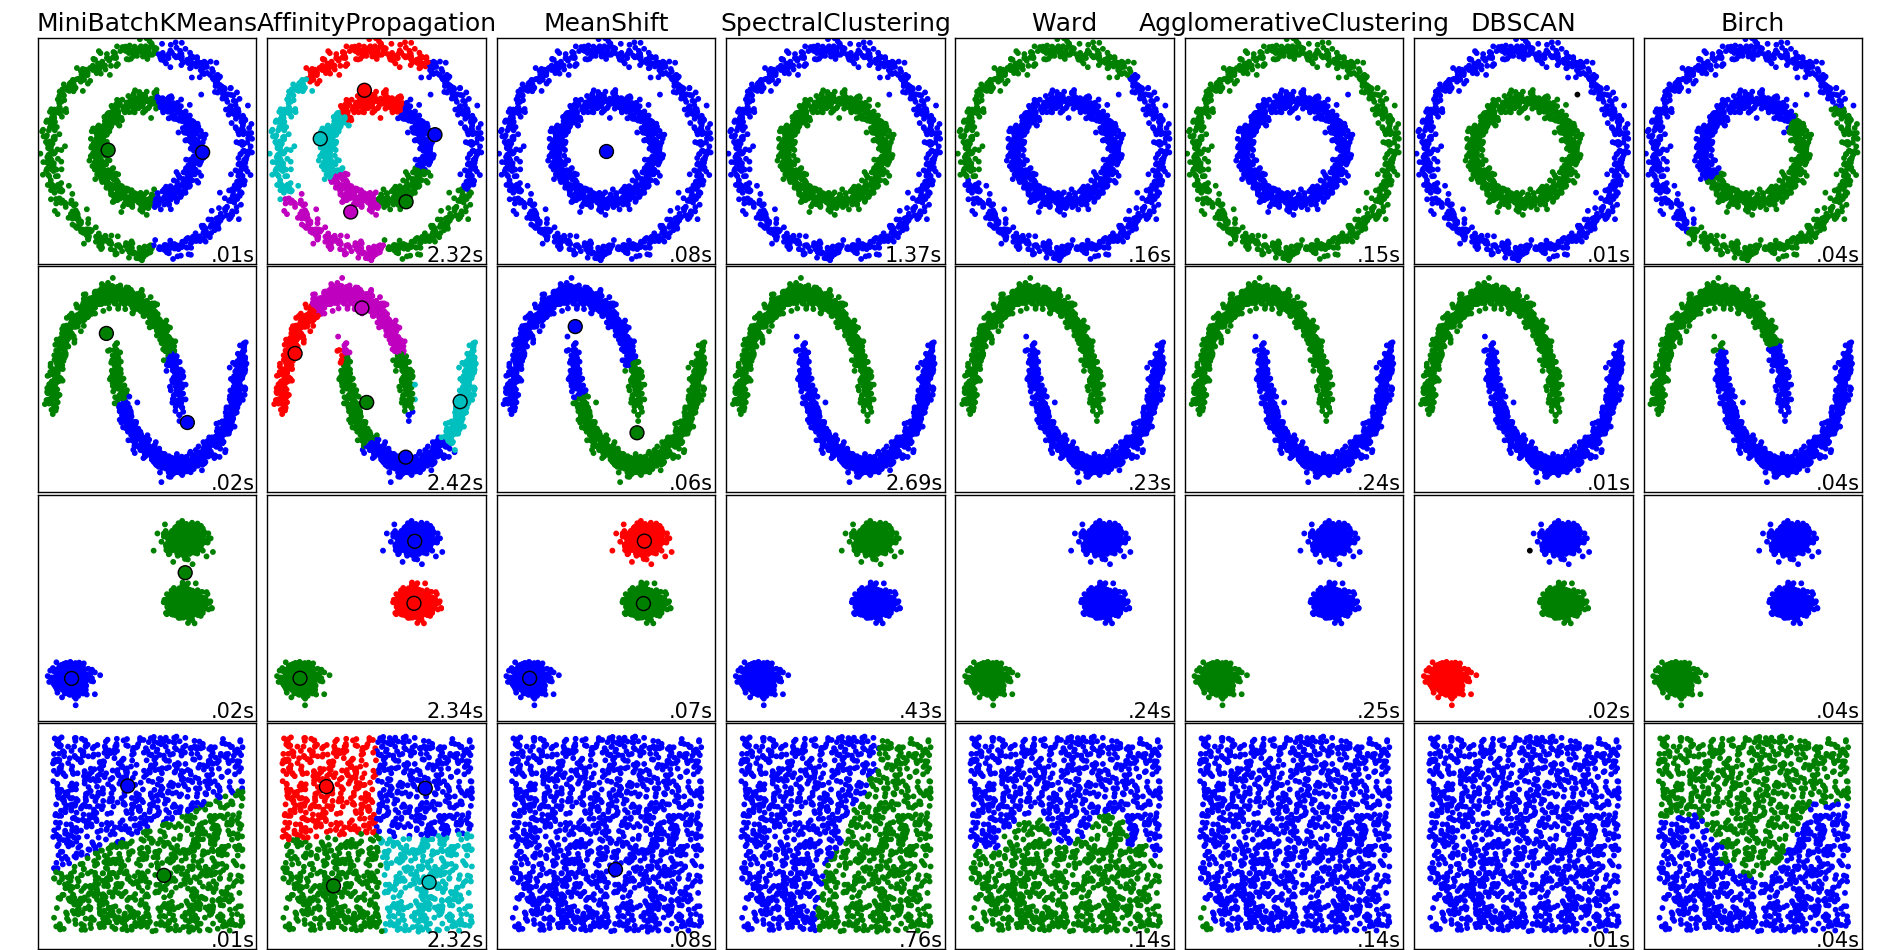
\includegraphics[width = 12cm,height = 7cm]{image/111.png}
% \caption{Comparing different clustering Algorithms }
% \label{dataclu}
% \end{figure}



%%---------------GHALAT ELMI-----------------------------------------------
% Streams consist of data tuples that need to be processed as they arrive, and mining these streams is challenging since the data distribution underlying
% a stream can evolve significantly over time. Besides dealing with evolving distributions, stream clustering algorithms have to meet several technical requirements, including limited time, limited memory, and processing the stream in a single pass. A multitude of stream clustering algorithms has been proposed in the literature that satisfy these requirements. 

% Of major importance is the quality of the resulting clustering, which can be measured by evaluation measures, also termed criteria, indices, validation measures, or validation indices.

%%-----------------------------------------------------------


%summery of conclusion

\section{Research Objectives}

The overall research goal is to improve current streaming AP models to generate micro and macro clusters from indoor localization data. The objectives can be described as follows. 

\begin{itemize}

    \item Develop a new data stream AP model (DSAP) for uncovering evolutionary patterns based on an online micro-cluster phase and offline macro-cluster phase.
     \item Apply the landmark time window model to continuously accumulate sufficient data points for computing the micro-clusters, avoiding performance issues.
    \item Evaluate the clustering results using performance and validation metrics that can be used to infer the advantages and limitations of the proposed DSAP model.  
    %\item Analyze the behavioral pattern in indoor localization experiments.
    \item Demonstrate the potential of DSAP for analyzing localization data streams in order to understand staircase usage patterns as well as occupant behavior in indoor spaces.
\end{itemize}  
    % \item Apply the online-offline phases of such a model to analysing indoor positioning stream data.  
    % \item Applying two data related to indoor localization positioning 
    %has certainly not been applied 
    % \item Apply streaming AP clustering algorithm to compare the proposed model and evaluate our model.

    %\item The proposed method is based on unsupervised learning, and data clustering. Affinity Propagation (AP) is a clustering message passing algorithm proposed by Frey and Dueck. This algorithm is selected for its properties of stability and of the way it represented each data cluster. The consequence of using AP is quadratic computational complexity, especially on large scale datasets.




 

%\section{Research Questions}


%The research questions of this research work are: 
% \begin{itemize}
%     \item Is streaming AP more suitable than streaming K-means for analysing e-counter data? 
%     \item Maintain a continuously consistent good clustering of the sequence observed so far, using a small amount of memory and time.

% \end{itemize}


\section{Scientific Contributions}


The main scientific contributions of this research work are summarized as follow:

\begin{itemize}
    %\item  extend a partitional clustering technique that can adapt to appearing or disappearing concepts in underlying data, thus achieving similar or better quality and performance of clustering than less-flexible techniques without requiring a specific level of clustering to use. NOT CLEAR WHAT YOU MEANT HERE
    
    \item A new data stream AP clustering (DSAP) algorithm is proposed for uncovering evolutionary patterns using the landmark time window model. Previous research work was focused on using the sliding time window model.
    
    \item  To the best of our knowledge, the streaming AP clustering algorithms have never been used for clustering indoor localization data streams before. 
    
    \item We demonstrate the potential of applying streaming cluster analysis to find new insights into stair usage and occupant behaviour in indoor spaces.
\end{itemize}


%\todo[inline]{}research premises 
%As far as we had research, there is not any research work present with affinity propagation used landmark time window model.


\section{Organization of this Thesis}
This thesis is organized in five chapters as described as follows:

Chapter 2 provides an overview of clustering methods by reviewing the various concepts, methods, and underlying steps, with a particular focus on the affinity propagation (AP) method.  Data stream clustering algorithms are also introduced with the time window models that are used for computing stream clusters.

Chapter 3 summarizes the related work in streaming AP clustering.

Chapter 4 describes the research methodology adopted for developing, implementing, and evaluating the proposed Data Stream Affinity Propagation (DSAP)algorithm using the landmark time window model. 

Chapter 5 describes the  design  and  implementation  of  the  DSAP  algorithm. Two  experiments  are  presented  that  are  related  to  applying  the proposed DSAP model to find stair usage patterns and occupant behaviour in indoor spaces.

Chapter 6 provides an in-depth discussion of the main  clustering  results  from  applying DSAP using  the  data  streams  generated  from  both  experiments. 

Finally, Chapter 7 concludes the work and outlines future research work.
% \end{document}






%There are challenges to designing a data stream platform, such as unbounded data or no control over the data arrival.

%%%%%%%%%%%%%%%%%%%%%%%%%%%%%%%%%%%%%%%
% Although AP still does not guarantee global optimum, several experiments in [13] have shown its consistent superiority over the previous algorithms. However, AP clustering has a limitation that it is hard to determine the value of parameter ‘preference’, which can lead to a suboptimal clustering solution.